\documentclass[journal,12pt,twocolumn]{IEEEtran}
\usepackage{graphicx}
\graphicspath{{./figs/}}{}
\usepackage{amsmath,amssymb,amsfonts,amsthm}
\newcommand{\myvec}[1]{\ensuremath{\begin{pmatrix}#1\end{pmatrix}}}
\newcommand*{\permcomb}[4][0mu]{{{}^{#3}\mkern#1#2_{#4}}}
\newcommand*{\perm}[1][-3mu]{\permcomb[#1]{P}}
\newcommand*{\comb}[1][-1mu]{\permcomb[#1]{C}}
\usepackage{listings}
\usepackage{watermark}
\usepackage{titlesec}
\let\vec\mathbf
\providecommand{\pr}[1]{\ensuremath{\Pr\left(#1\right)}}
\providecommand{\cbrak}[1]{\ensuremath{\left\{#1\right\}}}
\providecommand{\sbrak}[1]{\ensuremath{{}\left[#1\right]}}
\providecommand{\brak}[1]{\ensuremath{\left(#1\right)}}


\titlespacing{\subsection}{0pt}{\parskip}{-3pt}
\titlespacing{\subsubsection}{0pt}{\parskip}{-\parskip}
\titlespacing{\paragraph}{0pt}{\parskip}{\parskip}
\newcommand{\figuremacro}[5]{
    
}
\lstset{
frame=single, 
breaklines=true,
columns=fullflexible
}
\thiswatermark{\centering \put(0,-105.0){
\includegraphics[scale=0.4]{iith.png}} }

\sloppy
\title{\mytitle}
\title{
Digital Communication Assignment
}
\author{Nikhil Nair}
\begin{document}
\maketitle
%\tableofcontents
\bigskip


\section{\textbf{Problem }}
Generate samples of 
\begin{equation}
V = -2\ln\brak{1-U}  \nonumber
\end{equation}
and plot its CDF. 

\section{\textbf{Solution }}
The following code generates samples and plots the CDF of $V$.

\begin{lstlisting}
https://github.com/nikhilnair90/FWC/tree/main/Module-II/Digital Comm./6.3.1/Code/6_3_1.py
\end{lstlisting}



\section{\textbf{Figure }}
\begin{figure}[h]
    \centering
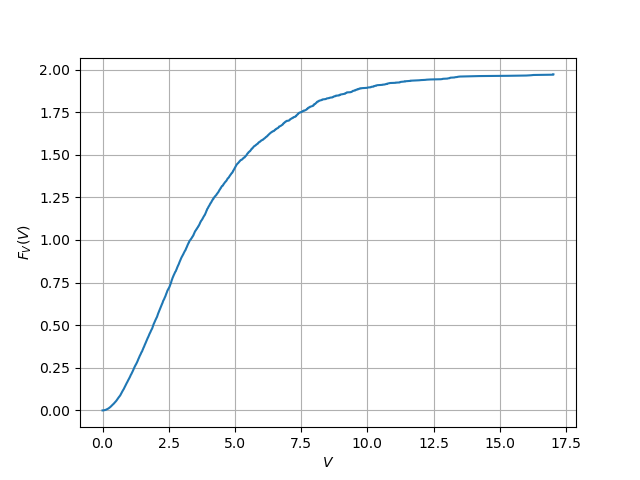
\includegraphics[width=\columnwidth]{figure/6_3_1.png}
    \label{fig:my_label}
\end{figure}

\end{document}
